\section{D\'efinition de quelques concepts m\'etiers}
\subsubsection{\textbf{Sinistre}}
Un sinistre est la réalisation de l'événement couvert par le contrat et qui donne lieu aux prestations assurées : indemnité, capital ou rente, assistance…
\subsubsection{\textbf{Charge d'un sinistre}}
 On d\'efinit la \textbf{charge} d'un sinistre, comme \'etant le co\^ut total du sinistre. Elle repr\'esente le montant que l'assureur doit payer \`a l'assur\'e. 
 
 \subsubsection{\textbf{Provision d'un sinistre}}
 La \textbf{provision} quant \`a elle, est l'ensemble des montants accumul\'es par l'entreprise d'assurances et de r\'eassurance pour faire face \`a ses engagements envers les assur\'es et b\'en\'eficiaires de contrats d'assurance. 
 
 \subsubsection{\textbf{R\`eglement du sinistre}}
 Le \textbf{r\`eglement} d'un sinistre d\'esigne le montant vers\'e comme indemnit\'e par l'assureur \`a l'assur\'e. 
 
 \subsubsection{\textbf{Recours}}
 Le \textbf{recours} quant à lui est une action amiable (lettres, mise en demeures) ou judiciaire (assignation), entreprise par la victime et/ou l'assureur contre le(s) responsable(s) du pr\'ejudice subi et/ou assureur dans le but d'\^etre d\'edommag\'e. On parle de recours \'emis, lorsqu'on se positionne du c\^ot\'e de la partie émettrice du recours. On parlera de recours subis lorsqu'on se place du c\^ot\'e de la partie qui reçoit le recours. 
 
 \subsubsection{\textbf{B\'en\'eficiaire}}
 Le b\'en\'eficiaire est une tierce personne physique ou morale, au profit de laquelle l'assurance a été contractée. Elle peut être nommément désignée aux conditions particulières du contrat ou bien apparaître dans les conditions générales sous les termes de : conjoint, p\`ere, m\`ere, ...
 
 
\section{Évaluation de la qualité de la donnée de la \acrlong{df}}
La premi\`ere phase de notre projet consistait \`a prendre en main Apache Griffin, afin de le configurer pour qu'il puisse r\'epondre aux besoins de la \acrshort{df}. Une fois achev\'ee,  la deuxi\`eme phase du projet a pour but d'\'evaluer \`a l'aide de l'outil, la qualit\'e des donn\'ees du socle, et de proposer des mesures de redressement lorsque cela est possible. \`A cet effet, deux extractions de donn\'ees ont \'et\'e fournies. Il s'agit des tables 'Detail\_Victimes' et 'Inventaire\_Sinistre'. La table 'Detail\_Victimes' contient les informations de toutes les victimes décédées ou blessées ainsi que l'historique des évaluations. La table 'Inventaire\_Sinistre' quant \`a elle contient tout l'inventaire du sinistre, y compris les règlements, les provisions, et les recours. Elles ont \'et\'e import\'ees dans PostgreSQL, suite \`a la cr\'eation d'une base de donn\'ees et la d\'efinition du sch\'ema des diff\'erentes tables. 


Au cours de l'importation, des anomalies ont \'et\'e d\'etect\'ees dont notamment la pr\'esence de chaîne de caract\`eres vide dans les colonnes '\emph{Resp}' des deux (2) tables. Ces colonnes sont cens\'ees contenir des donn\'ees num\'eriques. De plus, le format (JJ/MM/AAAA) de toutes les colonnes contenant des donn\'ees de type \textit{date} dans la table 'Inventaire\_Sinistre', \'etait incompatible avec le format attendu par PostgreSQL (AAAA-MM-JJ). Afin de contourner ces diff\'erentes difficult\'es, nous avons import\'e les colonnes '\emph{Resp}' au format \textit{varchar(100)}, remplac\'e les chaînes de caract\`eres vide par \textit{null} puis proc\'ed\'e \`a un transtypage au format \textit{real}. De m\^eme, pour les colonnes contenant des dates, nous avons proc\'ed\'e \`a une importation au format \textit{varchar(100)} puis un transtypage au format \textit{date},le tout automatis\'e dans un script \acrshort{sql}. Une fois nos donn\'ees import\'ees dans PostgreSQL, nous avons r\'ealis\'e l'\'evaluation de la qualit\'e  de chaque table avec Griffin. Les r\'esultats sont pr\'esent\'es suivants chaque dimensions.

\subsection{Pr\'esentation des donn\'ees}
\begin{table}[H]
\caption{Composition des diff\'erentes tables}
{\footnotesize
\begin{center}
\begin{tabular}{llcc}
\toprule 
&& \textbf{Detail\_Victimes} & \textbf{Inventaire\_Sinistre} \\
\midrule
\textbf{Nombre de lignes} && 477 942 & 1 885 568 \\ 
\textbf{Nombre de colonnes} && 93 & 90 \\
\textbf{Attributs de type chaîne de caract\`eres} && 26 & 48 \\
\textbf{Attributs de type r\'eel} && 57 & 25 \\
\textbf{Attributs de type entier} && 2 & 6 \\
\textbf{Attributs de type date} && 8 & 11 \\
\bottomrule
\end{tabular}
\end{center}}
\end{table}

Nous allons \'egalement pr\'esent\'e quelques variables qui interviendront dans la suite.

%\begin{table}[h]
\topcaption{Quelques variables de la table 'Inventaire\_Sinistre'}
%\vspace{0.5cm}
{\footnotesize
\begin{center}
\begin{supertabular}{lcl}
\toprule 
& \textbf{Inventaire\_Sinistre} &  \\
\midrule
\textbf{Variable}                                 & \textbf{Type}                         & \textbf{Description}  \\
\hline 
\textbf{NUMERO\_SINISTRE}                          & Cha\^ine de caract\`eres    & Identifiant du sinistre   \\ 
DATE\_SURVENANCE                          & Date                        & Date survenance du sinistre   \\ 
DATE\_DECLARATION                         & Date                        & Date Déclaration du sinistre   \\ 
DATE\_OUVERTURE                           & Date                        & Date Ouverture du dossier sinistre   \\ 
DATE\_CLOTURE                             & Date                        & Date Clôture du dossier sinistre\\ 
DATE\_NAISSANCE\_CONDUCTEUR               & Date                        & Date de naissance du conducteur   \\ 
DATE\_PERMIS                              & Date                        & Date du permis\\ 
CHARGE                                    & R\'eel                      & Coût total du sinistre   \\ 
PROVISION\_TOTAL                          & R\'eel                      & Provision du sinistre   \\ 
REGLEMENTS\_TOTAL                         & R\'eel                      & Reglements du sinistre   \\ 
VICTIMES\_BLESSEES                        & Entier                     & Nombre de victimes blessées dans le sinistre \\
VICTIMES\_DECEDEES                        & Entier                     & Nombre de victimes décédées dans le sinistre\\
NATURE\_SINISTRE                          & Cha\^ine de caract\`eres    & Nature du sinistre (corporel ou materiel) \\
\bottomrule
\end{supertabular}
\end{center}}

%\end{table}

\begin{table}[H]
\caption{Quelques variables de la table 'Detail\_Victime'}
%\vspace{0.5cm}
{\footnotesize 
\begin{center}
\begin{tabular}{lcl}
\toprule 
& \textbf{Detail\_Victimes} &  \\
\midrule
\textbf{Variable}                                 & \textbf{Type}                         & \textbf{Description}  \\
\hline 
NUMERO\_SINISTRE                          & Cha\^ine de caract\`eres    & Identifiant du sinistre   \\ 
DATE\_SURVENANCE                          & Date                        & Date survenance du sinistre   \\ 
DATE\_DECLARATION                         & Date                        & Date Déclaration du sinistre   \\ 
BENEFICIAIRE                             & Cha\^ine de caract\`eres     & Désigne le b\'en\'eficiaire   \\ 
FRAISMEDPHARMA                           & R\'eel                       & \acrfull{fmp} \\
RSK\_FMPVALINIT\_IND                     & Cha\^ine de caract\`eres     & Indicateur \acrshort{fmp}(Y/N)\\
MONTANT\_IPP                             & R\'eel                       & Montant \acrfull{ipp}\\
RSK\_IPPVALINIT\_IND                     & Cha\^ine de caract\`eres     & Indicateur \acrshort{ipp}(Y/N)        \\
NATUREDESDEGATS                          & Cha\^ine de caract\`eres     & Nature des d\'egats(Bless\'e,Mortel) \\
NATURE\_SINISTRE                          & Cha\^ine de caract\`eres     & Nature du sinistre (corporel ou materiel) \\
VICTIMEKEY                               & Cha\^ine de caract\`eres     & Identifiant de la victime \\
\bottomrule
\end{tabular}
\end{center}}

\end{table}


\normalfont
\subsection{Dimension de Compl\'etude} 
Nous utilisons ici trois (3) m\'etriques pour appr\'ecier cette dimension: le nombre total de lignes, le nombre d'observations incompl\`etes et le nombre d'observations non nulles. Elles sont calcul\'ees comme suit: 
\begin{lstlisting}[language=SQL,caption={R\`egles de la Dimension Compl\'etude},captionpos=t ,showspaces=false,basicstyle=\scriptsize,numbers=none,commentstyle=\color{gray},backgroundcolor=\color{background}]
--total : 
SELECT COUNT(*) AS total FROM source, save as table total_count

--nombre d'enregistrements incomplets: 
SELECT COUNT(*) as incomplete FROM source 
WHERE NOT (numero_contrat IS NOT NULL), save as table incomplete_count

--nombre d'enregistrement complets: 
SELECT (total_count.total - incomplete_count.incomplete) AS complete 
FROM source LEFT JOIN incomplete_count, save as table complete_count
\end{lstlisting}
Cette dimension est ex\'ecut\'ee pour toutes les colonnes des deux tables. Nous avons obtenu les r\'esultats suivants:  
\begin{itemize}[parsep=0cm,itemsep=0cm]
\item table 'Detail\_Victimes': quatre-vingt (80) colonnes ont des valeurs manquantes (soit environ 86\%) dont cinq (5) compl\`etement vides, dix (10) ayant \`a peine 10\% de valeurs compl\`etes et vingt (20) avec un taux de valeurs manquantes compris en 20 et 50\%;
\item table 'Inventaire\_Sinistre': on compte trente-neuf (39) colonnes avec des valeurs manquantes (soit environ 43\%) dont cinq (5) enti\`erement nulles et six (6) avec plus de 30\% de valeurs nulles.
\end{itemize}
Voici un aperçu du tableau de bord:
\begin{figure}[H]
        \caption{Visualisation de la dimension Compl\'etude pour la table 'Detail\_Victimes'}  \label{fig:tttay}
    %\advance\rightskip-2cm
    %\advance\leftskip-4cm
    \begin{center}
      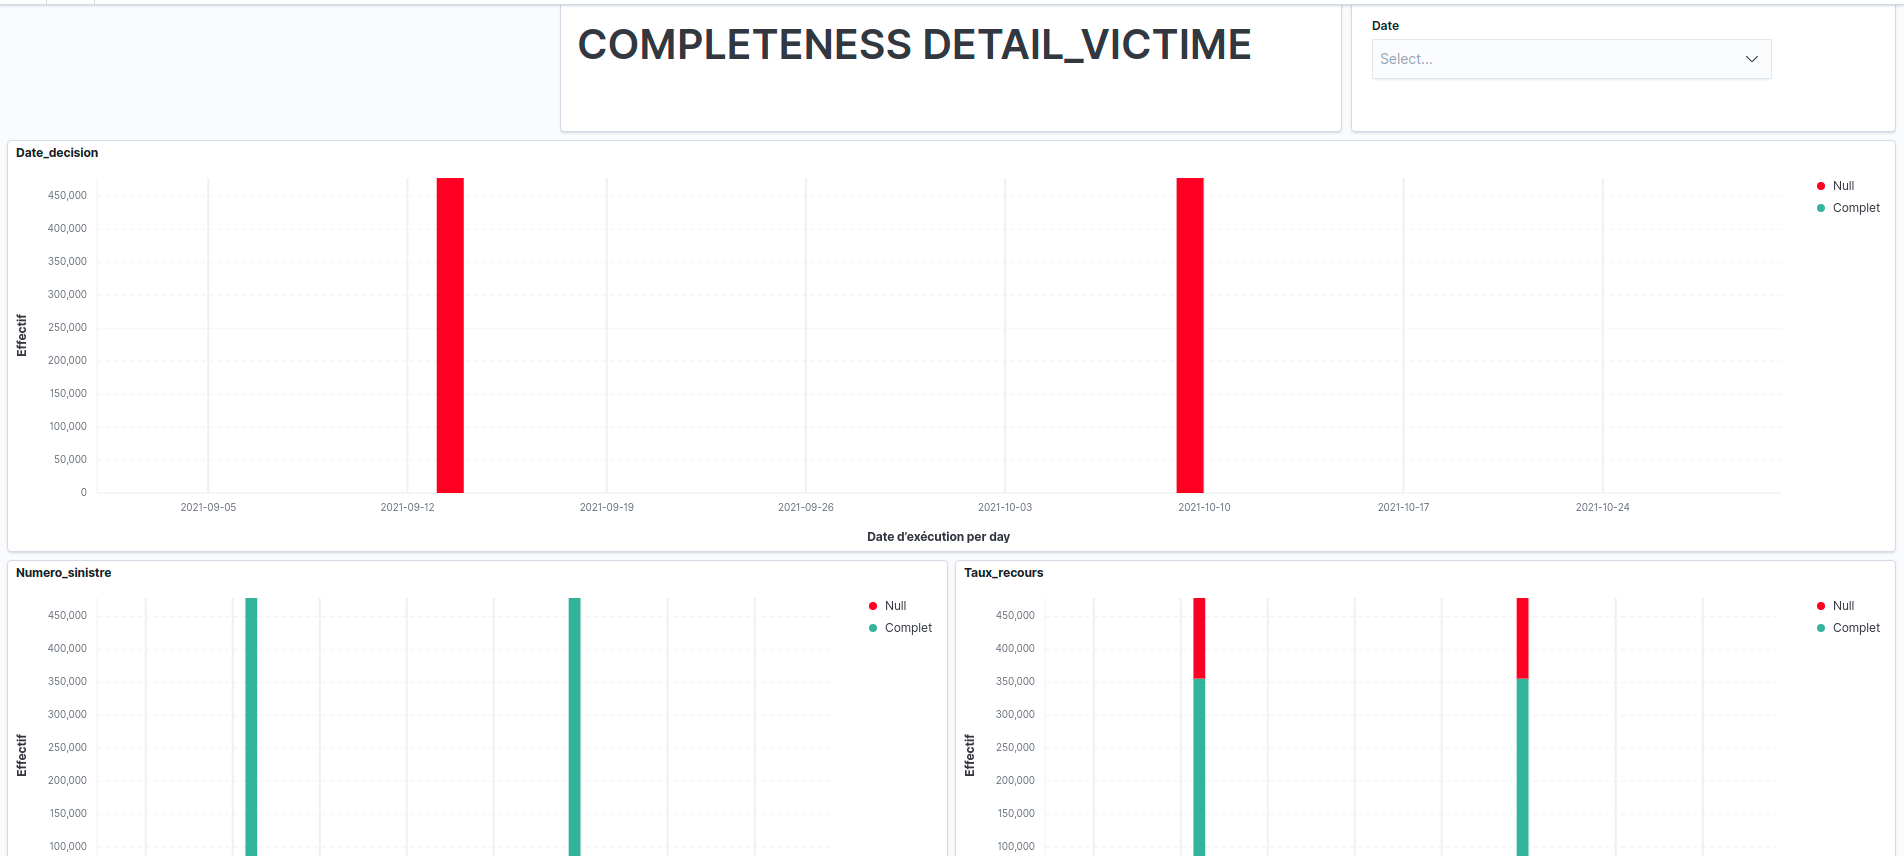
\includegraphics[scale = 0.27]{Main/Static/Completeness_Detail_Victime.png} 
    \end{center}
\end{figure}
Toutefois, toutes les colonnes pr\'esentant des valeurs manquantes n'ont pas pour autant des probl\`emes de qualit\'e. Il peut s'agir d'une r\'eponse inappropri\'ee au regard du contexte. Afin de pousser plus loin l'\'evaluation de la qualit\'e, une analyse de la p\'eriode couverte par ces valeurs manquantes fut faite au niveau de la dimension de coh\'erence.

\subsection{Dimension d'Unicit\'e}
Pour cette dimension, nous avons \'egalement fait ressortir pour chaque colonne cibl\'ee trois (3) m\'etriques :  le nombre total d'observations dans la colonne, le nombre d'observations distinctes et le nombre d'observations distinctes apparaissant plus d'une fois. Les r\`egles ayant permis d'obtenir ces m\'etriques sont les suivantes : 
\newpage
\begin{lstlisting}[language=SQL,caption={R\`egles de la Dimension Unicit\'e},captionpos=t,showspaces=false,basicstyle=\scriptsize,numbers=none,commentstyle=\color{gray},backgroundcolor=\color{background}]
--total_numero_contrat et distinct_numero_contrat: 
SELECT COUNT(src.numero_contrat) AS total_numero_contrat, 
COUNT(DISTINCT src.numero_contrat) as distinct_numero_contrat FROM src 

--duplicated_numero_contrat: 
SELECT COUNT(tmp.numero_contrat) as duplicated_numero_contrat 
FROM (SELECT numero_contrat FROM src GROUP BY numero_contrat 
HAVING COUNT(numero_contrat) > 1) as tmp
\end{lstlisting}

\begin{figure}[H]
        \caption{Visualisation de la dimension Unicit\'e pour la table 'Inventaire\_Sinistre'}  \label{fig:tttay}
    %\advance\rightskip-2cm
    %\advance\leftskip-4cm
    \begin{center}
      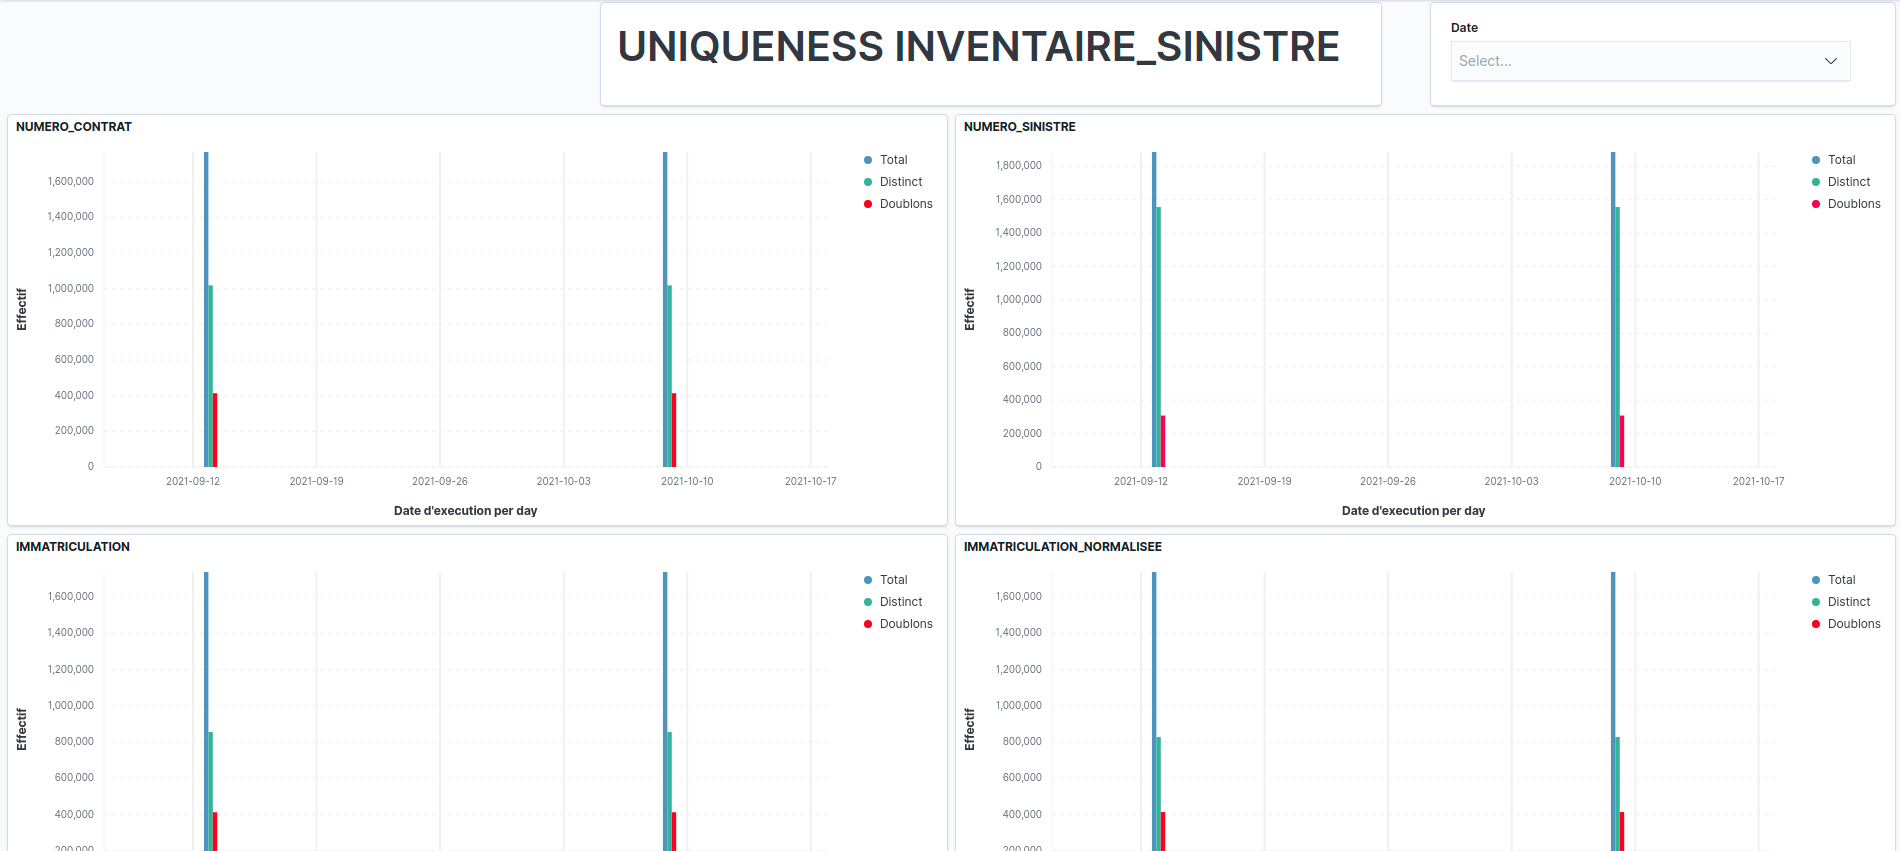
\includegraphics[scale = 0.27]{Main/Static/Uniqueness_Inventaire_Sinistre.png} 
    \end{center}
\end{figure}
Ces r\`egles sont appliqu\'ees, sur des colonnes pr\'esentant \`a priori des contraintes d'unicit\'e ou repr\'esentant des num\'eros ou codes d'identification. Les r\'esultats issus de cette \'evaluation ont r\'ev\'el\'e qu'il y avait des r\'ep\'etitions au niveau des diff\'erentes colonnes. Mais cela ne constituait pas n\'eanmoins des anomalies. Cela s'explique par le fait que les donn\'ees sont issues de la jointure entre plusieurs tables.


\subsection{Dimension de Validit\'e} 
Au niveau de cette dimension nous avons \'evalu\'e trois (3) grandes r\`egles. L'objectif \'etait d'identifier la plage de variation des colonnes quantitatives, de d\'efinir les modalit\'es des diff\'erentes colonnes qualitatives et de faire ressortir les valeurs pr\'esentant des probl\`emes d'encodages de caract\`eres accentu\'es. Essentiellement les r\`egles \'evalu\'ees sont les suivantes : 
\newpage
\begin{lstlisting}[language=SQL,caption={R\`egles de la Dimension Validit\'e},captionpos=t,showspaces=false,basicstyle=\scriptsize,numbers=none,commentstyle=\color{gray},backgroundcolor=\color{background}]
--plage de valeurs numeriques (griffin-dsl): 
min(montant_evaluation) as montant_evaluation_minimal,
max(montant_evaluation) as montant_evaluation_maximal, 
avg(montant_evaluation) as montant_evaluation_moyenne

--differentes modalites:
SELECT DISTINCT(classe_victime) AS classe_victime_distinct from src

--detection des problemes d'encodage:
SELECT DISTINCT(beneficiaiare) FROM src 
WHERE beneficiaiare rlike '[a-zA-Z]+[?]+[a-zA-Z]*'
\end{lstlisting}
Suite \`a l'\'evaluation de cette dimension, nous avons mis en \'evidence comme anomalie des probl\`emes d'encodages dans la colonne '\textit{Beneficiaire}' de la table 'Detail\_Victimes'.  Les probl\`emes d'encodages tels que nous les avons d\'etect\'es sont caract\'eris\'es par l'apparition de '?' en lieu et place des caract\`eres accentu\'es. Ainsi p\`ere se retrouve écorché en 'p?re' par exemple.
\begin{figure}[H]
        \caption{Visualisation de la dimension Validit\'e pour la table 'Detail\_Victimes'}  \label{fig:tttay}
    %\advance\rightskip-2cm
    %\advance\leftskip-4cm
    \begin{center}
      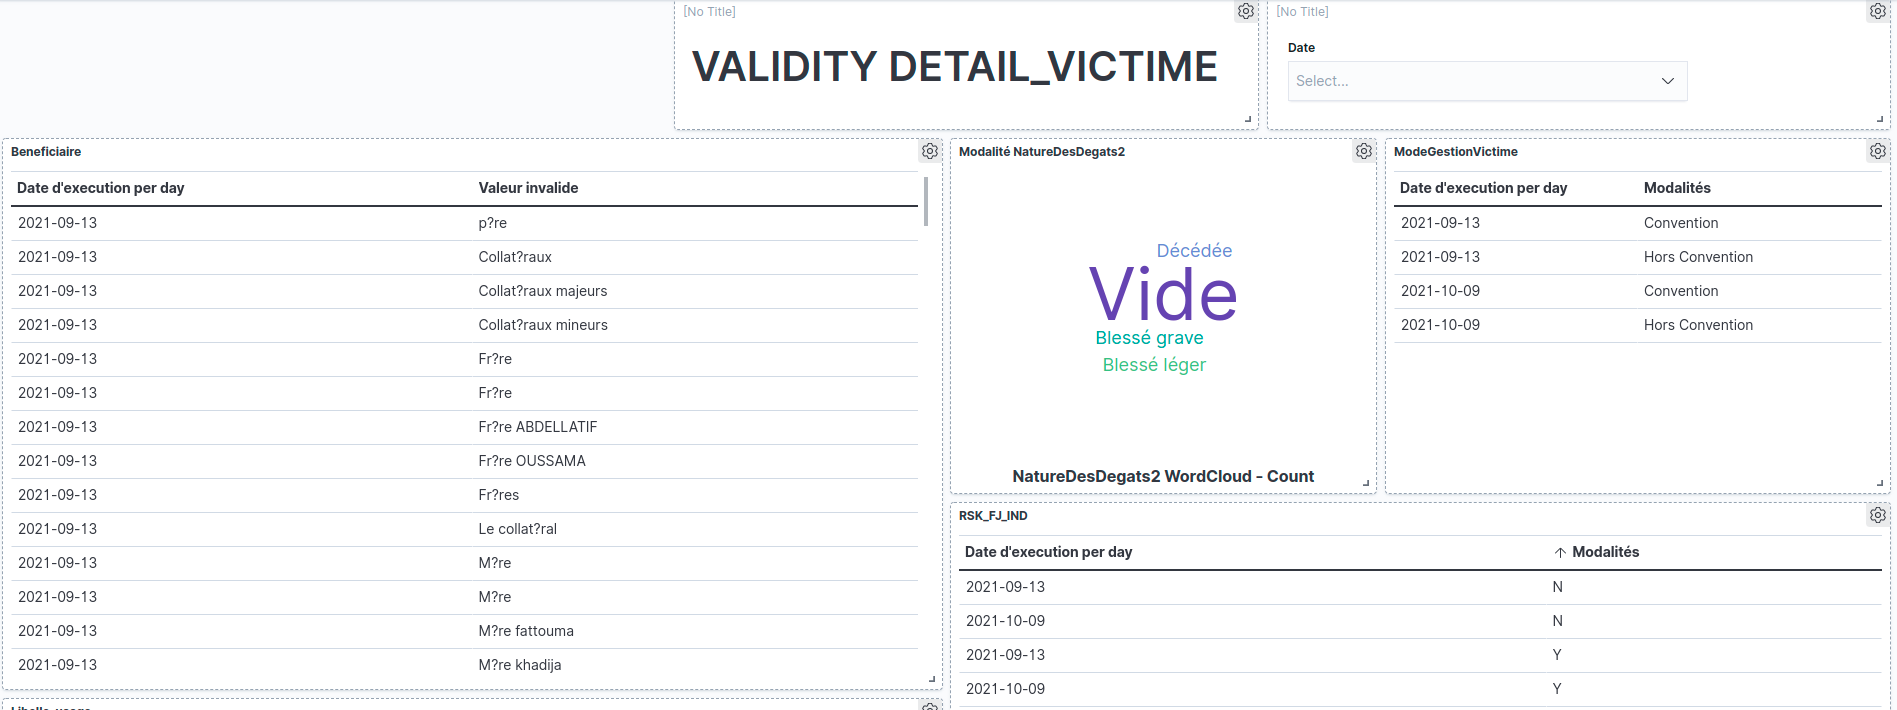
\includegraphics[scale = 0.27]{Main/Static/Validity_Detail_Victime.png} 
    \end{center}
\end{figure}

% De plus, bien que des valeurs n\'egatives aient \'et\'e d\'etect\'ees pour des variables repr\'esentant des montants, il s'est av\'er\'es que ces valeurs \'etaient utilis


\subsection{Dimension de Coh\'erence }
\subsubsection{\textbf{Table 'Inventaire\_Sinistre'}}
Les r\`egles \'etablies au niveau de cette dimension, permettent d'attester de la coh\'erence des donn\'ees vis-\`a-vis des r\`egles m\'etiers. La table 'Inventaire\_Sinistre' permet de capter les informations relatives \`a un sinistre, comme le co\^ut, le nombre de victimes, les dates cl\'es... On s'attend \`a ce que les formules actuarielles suivantes soient respect\'ees:
%\begin{equation}
%Charge = Provisions + Reglement - Recours\_encaissé - Recours\_a\_encaissé
%\end{equation}

\begin{equation}
  \begin{split}                                  
   Charge\_sinistre =  Reglement\_garantie + Reglement\_intervenant - \\
       Recours\_emis\_recuperer + Recours\_subis\_payer + \\
       Provisions\_garanties +  Provision\_intervenant - \\
        Provision\_recours\_emis + Provision\_recours\_subi -\\
        Recours\_emis + Recours\_subis
  \end{split}
\end{equation}

\begin{equation}
\begin{split}  
	Reglement\_total =  Reglement\_garantie + Reglement\_intervenant 
 \end{split}
\end{equation}

 
\begin{equation}
\begin{split}  
 Provisions\_total = Provisions\_garantie\_actuel + \\
 Provisions\_intervenant\_actuel  
\end{split}
\end{equation}
 Elles ont permis d'\'elaborer des r\`egles de qualit\'es. En effet, la coh\'erence au niveau de la charge repr\'esente une grosse probl\'ematique au sein de la \acrshort{df}. Nous avons \'egalement v\'erifi\'e la coh\'erence au niveau des dates. Logiquement, les date de survenance du sinistre, date d'ouverture du dossier et date de naissance du conducteur, doivent respectivement \^etre ant\'erieures aux date de d\'eclaration du sinistre, date de clôture et date de permis. Des incoh\'erences d\'etect\'ees \`a ce niveau, peuvent permettre de d\'eceler des cas de fraudes.\\

Par ailleurs, un sinistre peut \^etre qualifi\'e de Corporel, 'Materiel' ou 'Mixte' suivant la nature des d\'eg\^ats qu'il a provoqu\'e chez les victimes. Dans la table, seuls les sinistres de nature 'Corporel' et 'Materiel' sont pr\'esents. Ainsi, un sinistre ayant provoqu\'e des blessures et/ou caus\'e des pertes en vies humaines ne peut \^etre qualifi\'e de 'Materiel'. Ce qui est tout \`a fait logique. De m\^eme, certains sinistres peuvent \^etre affect\'es du qualificatif 'Corporel', s'ils ont co\^ut\'e plus de 100 000 dirham marocain bien qu'il n'y ait ni bless\'e ni mort. Ces diff\'erentes r\`egles permettent d'\'evaluer la coh\'erence des informations contenues dans les colonnes '\textit{Victimes\_Decedees}', '\textit{Victimes\_Blessees}' et '\textit{Nature\_Sinistre}'. Aussi, avec la table 'Detail\_Victime' qui contient les informations des diff\'erentes victimes d'un sinistre, on doit pouvoir retrouver le nombre total de victimes (bless\'ees ou d\'ec\'ed\'ees) de chaque sinistre dans l'inventaire. En plus de ces r\`egles, une attention particuli\`ere est port\'ee sur certaines colonnes afin d'identifier la p\'eriode couverte par les valeurs nulles. Un extrait des r\`egles se pr\'esente comme suit : 
\newpage
\begin{lstlisting}[language=SQL,caption={R\`egle de la Dimension Coh\'erence pour la table \textit{Inventaire\_Sinistre}},captionpos=t,showspaces=false,basicstyle=\scriptsize,numbers=none,commentstyle=\color{gray},backgroundcolor=\color{background}]
--regle de verification des formules: 
	--nombre d'enregistrements incoherents:
SELECT COUNT(*) FROM src WHERE 
power((reglements_total - reglement_garantie+reglement_intervenant),2)>1
	--echantillon incoherent
SELECT numero_sinistre, reglements_total, reglement_garantie,reglement_intervenant,
reglement_garantie+reglement_intervenant as somme_reglement 
FROM src 
WHERE power((reglements_total- reglement_garantie+reglement_intervenant),2)>1 
LIMIT 20

--regles de coherence des dates:
	--nombre d'enregistrements incoherents:
SELECT COUNT(*) AS nb_inconsitency_date_survenance_declaration FROM src 
WHERE date_survenance > date_declaration 
	--echantillon incoherent
SELECT numero_sinistre,date_survenance,date_declaration,statut_sinistre 
FROM src WHERE date_survenance > date_declaration LIMIT 20

--periode d'apparition des valeurs nulle:
SELECT MIN(date_creation_systeme), MAX(date_creation_systeme) FROM src 
WHERE COALESCE(numero_contrat,'empty') ='empty'

--regle de coherence nature_sinistre
SELECT COUNT(*) FROM  
(SELECT numero_sinistre FROM src WHERE nature_sinistre = 'Materiel' 
GROUP BY numero_sinistre HAVING SUM(victimes_blessees)> 0 
and SUM(victimes_decedees) >0)T

--regle de coherence nombre de victimes
SELECT COUNT(*) FROM 
(SELECT numero_sinistre, SUM(victimes_decedees) AS victimes_decedees 
FROM tgt GROUP BY numero_sinistre ) AS inventaire_sinistre ,
(SELECT numero_sinistre, COUNT(DISTINCT victime_key)  AS nb_decedees FROM src 
WHERE naturedesdegats = 'Mortel' GROUP BY numero_sinistre )T 
WHERE inventaire_sinistre.numero_sinistre = T.numero_sinistre 
AND inventaire_sinistre.victimes_decedees != T.nb_decedees
\end{lstlisting}
Plusieurs incoh\'erences ont pu \^etre d\'etect\'ees. Nous avons notamment:
\begin{itemize}[parsep=0cm,itemsep=0cm]
\item 1 sinistre de nature 'Materiel' mais avec 5 victimes bless\'ees et une d\'ec\'ed\'ee; 
\item 237 657 sinistres dont la charge est inf\'erieure \`a 100 000 dirham marocain, avec aucune victime enregistr\'ee mais de nature 'Corporel'; 
\item 190 622 sinistres dont le nombre de victimes est in\'egale au compte fait dans la table '\textit{Detail\_Victimes}';
\item 102 observations pour lesquelles le sinistre est d\'eclar\'e avant sa survenance;
\item 3 972 observations pour lesquelles la date d'obtention du permis de conduire est ant\'erieure \`a la date de naissance;
\item 76 000 observations ayant des dates d'ouverture de dossier chronologiquement post\'erieures \`a la date de clôture du dossier.
\end{itemize}

%sont caract\'eris\'ees par un ph\'enom\`ene de sinistre survenues apr\'es la d\'eclaration de sinistre a

\subsubsection{\textbf{Table 'Detail\_Victimes'}}
Cette table contient les informations li\'ees aux dommages corporels subis par les victimes d'un sinistre. Ces dommages occasionnent des frais. \`A cet effet, des variables indicatrices marquent la pr\'esence ou non de ces frais pour une victime donn\'ee. Donc un montant devrait \^etre enregistr\'e pour les \acrfull{fmp}, par exemple, uniquement si on indique que des frais ont \'et\'e occasionn\'es. Il en est de m\^eme pour l'\acrfull{ipp}. Il s'agit l\`a de l'une des v\'erifications de coh\'erence faites au niveau de cette table. Une v\'erification a \'egalement \'et\'e faite sur la coh\'erence des date de survenance et de d\'eclaration. On a donc les r\`egles suivantes:
\begin{lstlisting}[language=SQL,caption={R\`egle de la Dimension Coh\'erence pour la table \textit{Detail\_Victimes}},captionpos=t,showspaces=false,basicstyle=\scriptsize,numbers=none,commentstyle=\color{gray},backgroundcolor=\color{background}]
--incoherences frais medicaux et pharmaceutiques: 
	--si la variable indicatrice = N:
SELECT rsk_fmpvalinit_ind ,COUNT(*) as nb_incoherence_fmp_N, 
sum(fraismedpharma)/10000000 AS fraismedpharma 
FROM src WHERE rsk_fmpvalinit_ind = 'N' AND fraismedpharma > 0 
GROUP BY rsk_fmpvalinit_ind

	-- si la variable indicatrice est nulle
SELECT COALESCE(rsk_fmpvalinit_ind) AS rsk_fmpvalinit_ind , 
count(*) as nb_incoherence_fmp_null, sum(fraismedpharma)/10000000 
AS fraismedpharma FROM src WHERE rsk_fmpvalinit_ind is null 
AND fraismedpharma > 0 GROUP BY rsk_fmpvalinit_ind
\end{lstlisting}
L'ex\'ecution des r\`egles a permis de r\'ev\'eler les r\'esultats suivants: 
% pour  observations, des montants de frais medicaux et pharmaceutiques ont \'et\'e enregistr\'es tandis que la variable indicatrice marquait 'N'. De m\^eme, pour 4 761 observations manquantes de la variable indicatrice, un cumul de 6 6124 800 unit\'es mon\'etaires de frais medicaux et pharmaceutiques ont \'et\'e enregistr\'e. Pour ce qui est 

\begin{table}[H]
\caption{Point des incoh\'erences sur la table 'Detail\_victimes'}
{\footnotesize
\begin{center}
    
\begin{tabular}{llccc}
\toprule 
&& \textbf{Variable indicatrice} & \textbf{Enregistrements incoh\'erents} & \textbf{Montant cumul\'e}  \\
\midrule
\textbf{\acrshort{fmp}} && N & 6 892 & 66 124 800 \\ 
\textbf{\acrshort{fmp}} && Manquant & 4 761 & 57 652 924\\ 
\textbf{Montant \acrshort{ipp}} && N & 115 897 & 3 376 529 920 \\
\textbf{Montant \acrshort{ipp}} && Manquant & 59 602 & 1 891 223 296  \\
\bottomrule
\end{tabular}
\end{center}
}
\end{table}
En outre, 19 082 observations sont affect\'ees par une incoh\'erence entre les dates de survenance et de d\'eclaration.
\newpage